This is a ``conceptual'' question. You don't need to give formal proofs. Giving a text-based description, examples and/or pictures is fine.

\vspace{5mm}
Consider binary classification, with ${\cal{X}} = \mathbb{R}^d$ for some $d \geq 2$ and ${\cal Y} = \{-1,1\}$ and a  training dataset $\{(\xv_i,y_i)\}_{i \in [n]}$.


An enthusiastic student tries the following new approach towards training.
\begin{itemize}
    \item The student creates a new training dataset of $nd$ samples as follows.\\
    For each $i \in [n]$ and $j \in [d]$ define $\mathbf{z}_{ij} \in \mathbb{R}^{d}$ whose $j^{th}$ coordinate equals the $j^{th}$ coordinate of $\xv_i$ and all other coordinates are zero. The following figure shows an example:\\
    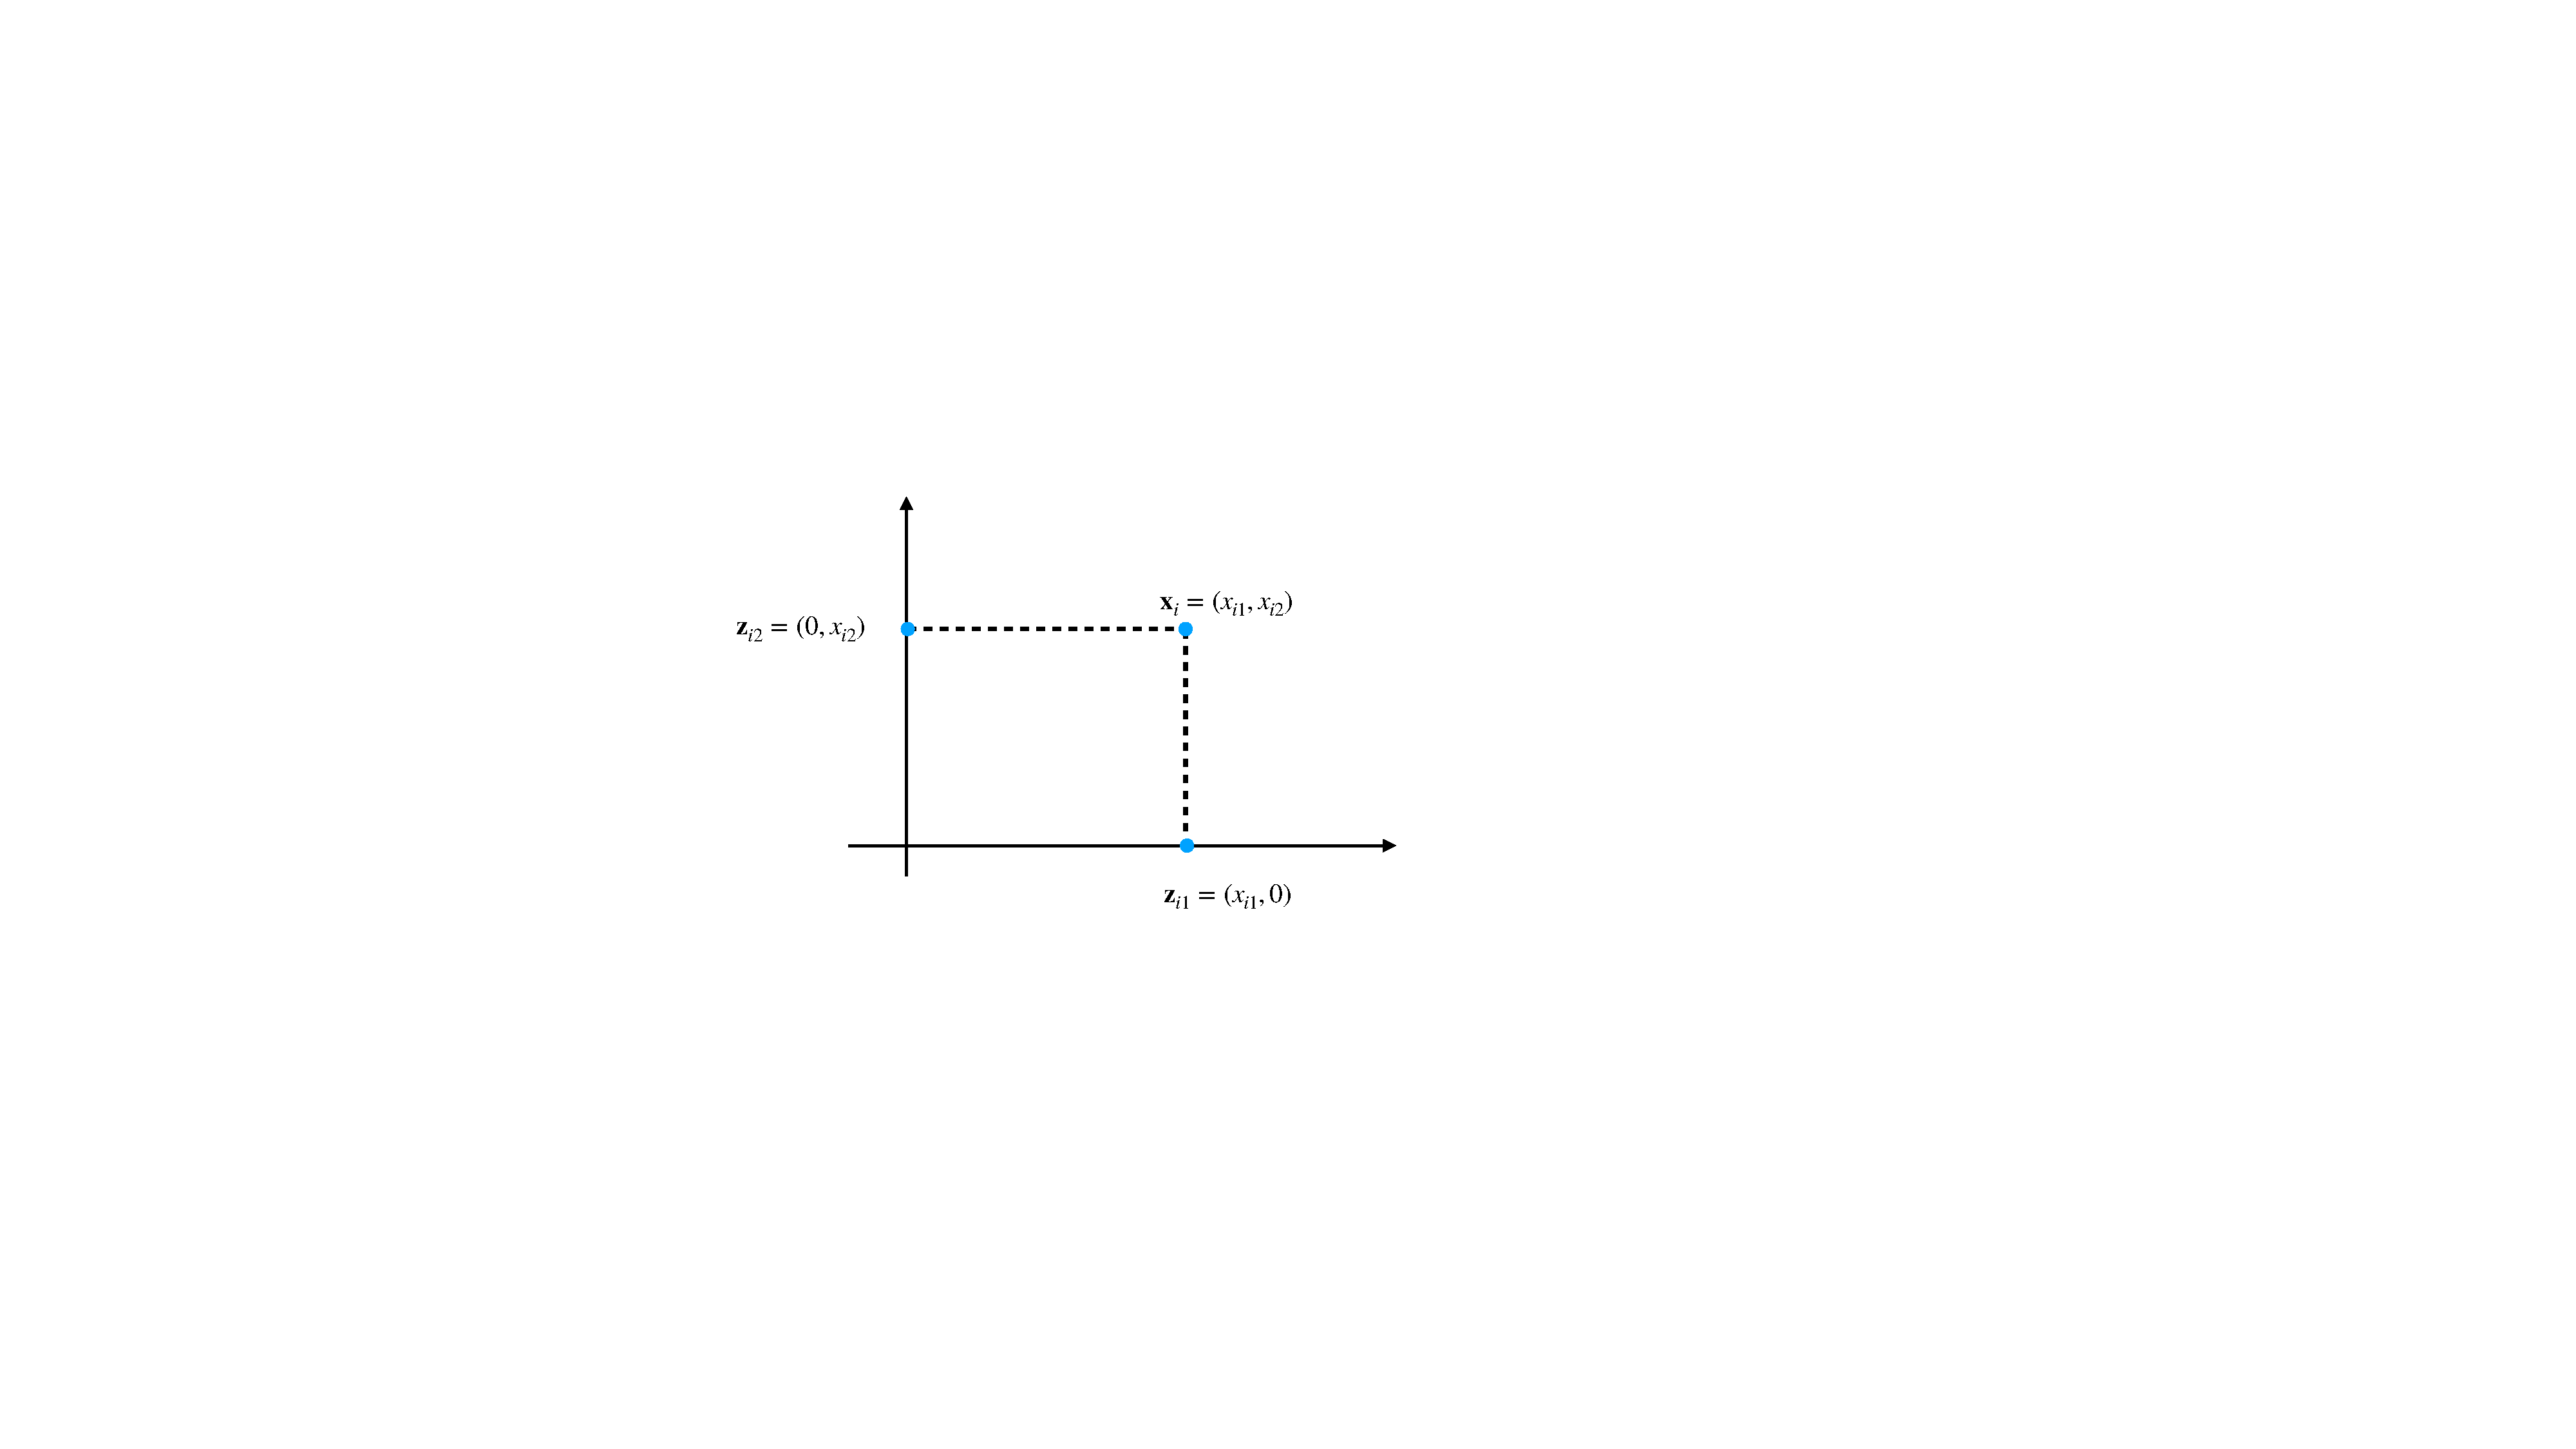
\includegraphics[width=0.5\linewidth]{midterm/images/enthusiastic.pdf}
    
     Now consider the modified training dataset:  $\{(\mathbf{z}_{ij},y_{ij})\}_{i\in [\,n\,]\; j\in [\,d\,]}$.

    \item The enthusiastic student trains a perceptron on this modified training set and obtains $\wv \in \mathbb{R}^d, b \in \mathbb{R}$.
    \item Given a new point $\xv \in \mathbb{R}^d$, the prediction is $f(\xv) = \text{sign} (\langle \wv, \xv \rangle + b)$.
\end{itemize}

\vspace{10mm}

What do you think about this idea? Are there settings where the perceptron algorithm can classify the original training data perfectly, but fails to do so on the modified training data? 

